\subsection{Critical section design}

\begin{theorem}{(170)} Critical section: \begin{itemize}
        \item 在critical section,CPU也可能被preempted。
        \item 滿足:\begin{itemize}
            \item Mutual exclusion:同一時間點,最多$1$ process在他的critical section,不允許多個processes同時在\textbf{各自}的critical section。
            \item Progress:不想進入critical section時,不能阻礙其他想進入critcal section的process進入,即不能參與進入critical section的decision,且必須在有限時間內決定進入critical section的process。
            \item Bounded waiting:Process提出申請進入critical section後,必須在有限時間內進入,即公平,NO starvation。
        \end{itemize}
        \item Busy waiting (spinlock) :若process平均可以在$<$ context switch時間內離開loop,則spinlock則有利。
        \item Busy waiting\textbf{無法}完全避免,在\code{Entry section}和\code{Exit section}仍是busy waiting實現,然而disable interrupt可以避免busy-waiting,但disable interrupt不適合multiprocessors。
    \end{itemize}
\end{theorem}

\subsubsection{Software support}

\begin{theorem}{(171)} Two processes solution:\begin{itemize}
        \item Algorithm 1(錯誤):\begin{itemize}
            \item 共享變數:\begin{lstlisting}[caption={Shared variables of Algorithm 1 (two processes solution).}, captionpos=b, mathescape=true]
                int turn := $i \lor j$
            \end{lstlisting}
            \item \textbf{Progress:不成立},當$P_i$在remainder section且$turn = i$,若$P_j$想進入critical section,但被$P_i$阻礙,須等到$P_i$進入critcal section再出來。
            \begin{algorithm}[H]
                \caption{$P_i$ of Algorithm 1 (two processes solution).}
                \begin{algorithmic}[1]
                    \Function{$P_i$}{}
                        \Repeat 
                            \While {$turn \neq i$}
                            \EndWhile
                            \State Critical section.
                            \State $turn$ := $j$
                            \State Remainder section.
                        \Until {$False$}
                    \EndFunction
                \end{algorithmic}
            \end{algorithm} 
            \begin{algorithm}[H]
                \caption{$P_j$ of Algorithm 1 (two processes solution).}
                \begin{algorithmic}[1]
                    \Function{$P_j$}{}
                        \Repeat 
                            \While {$turn \neq j$}
                            \EndWhile
                            \State Critical section.
                            \State $turn$ := $i$
                            \State Remainder section.
                        \Until {$False$}
                    \EndFunction
                \end{algorithmic}
            \end{algorithm} 
        \end{itemize}
        \item Algoroithm 2(錯誤):\begin{itemize}
            \item 共享變數:\begin{lstlisting}[caption={Shared variables of Algorithm 2 (two processes solution).}, captionpos=b, mathescape=true]
                // 表示是否想進入critical section。
                bool flag := $False$
            \end{lstlisting}
            \item \textbf{Progress:不成立},當$P_i, P_j$依序將$flag := True$,在\code{while}雙方皆會等待,則deadlock,皆無法進入critcal section。
            \begin{algorithm}[H]
                \caption{$P_i$ of Algorithm 2 (two processes solution).}
                \begin{algorithmic}[1]
                    \Function{$P_i$}{}
                        \Repeat 
                            \State $flag[i]$ := $True$
                            \While {$flag[j]$}
                            \EndWhile
                            \State Critical section.
                            \State $flag[i]$ := $False$
                            \State Remainder section.
                        \Until {$False$}
                    \EndFunction
                \end{algorithmic}
            \end{algorithm} 
            \begin{algorithm}[H]
                \caption{$P_j$ of Algorithm 2 (two processes solution).}
                \begin{algorithmic}[1]
                    \Function{$P_j$}{}
                        \Repeat 
                            \State $flag[j]$ := $True$
                            \While {$flag[i]$}
                            \EndWhile
                            \State Critical section.
                            \State $flag[j]$ := $False$
                            \State Remainder section.
                        \Until {$False$}
                    \EndFunction
                \end{algorithmic}
            \end{algorithm} 
        \end{itemize}
        \item Algorithm 3 (Peterson's solution)(正確):\begin{itemize}
            \item 共享變數:\begin{lstlisting}[caption={Shared variables of Peterson's solution (two processes solution).}, captionpos=b, mathescape=true]
                int turn := $i \lor j$
                bool flag := $False$
            \end{lstlisting}
            \item $flag$或$turn$或兩者值皆互換依然正確,但若將前兩行賦值順序對調,則因為mutual exclusion不成立,而不正確,可以通過hardware、OS support或high-level software APIs提供的synchronization tools。
            \item Peterson's solution is NOT guaranteed to work on modern PC, since processors and compiler may reorder read and write operations that have NO dependencies.
            \begin{algorithm}[H]
                \caption{$P_i$ of Peterson's solution (two processes solution).}
                \begin{algorithmic}[1]
                    \Function{$P_i$}{}
                        \Repeat 
                            \State $flag[i]$ := $True$
                            \State $turn$ := $j$
                            \While {$flag[j] \land turn = j$}
                            \EndWhile
                            \State Critacal section.
                            \State $flag[i]$ := $False$
                            \State Remainder section.
                        \Until {$False$}
                    \EndFunction
                \end{algorithmic}
            \end{algorithm}
            \begin{algorithm}[H]
                \caption{$P_j$ of Peterson's solution (two processes solution).}
                \begin{algorithmic}[1]
                    \Function{$P_j$}{}
                        \Repeat 
                            \State $flag[j]$ := $True$
                            \State $turn$ := $i$
                            \While {$flag[i] \land turn = i$}
                            \EndWhile
                            \State Critacal section.
                            \State $flag[j]$ := $False$
                            \State Remainder section.
                        \Until {$False$}
                    \EndFunction
                \end{algorithmic}
            \end{algorithm}
        \end{itemize}
    \end{itemize}
\end{theorem}

\subsubsection{Hardware support}

\begin{theorem}{()} Memory barrier (fence):\begin{itemize}
        \item Strongly ordered:對於memory修改 on $1$ processor is immediately visible to all other processers。
        \item Weakly ordered:對於memory修改 on $1$ processor may NOT be immediately visible to all other processers。
        \item System ensures that any L/S operations are completed before any subsequent L/S operations are performed.
    \end{itemize}
\end{theorem}

\begin{theorem}{(176)} Test-and-Set:\begin{itemize}
        \item \textsc{Test-and-Set}:
        \begin{algorithm}[H]
            \caption{Test-and-Set.}
            \begin{algorithmic}[1]
                \Function{Test-and-Set}{bool $*Target$} \Comment{Atomic.}
                \State bool $rv$ := $*Target$
                \State $*Target$ := $True$
                \State \Return $rv$
                \EndFunction
            \end{algorithmic}
        \end{algorithm}
        \item Algotihm 1(錯誤):\begin{itemize}
            \item 共享變數:\begin{lstlisting}[caption={Shared variables of Algorithm 1 (\textsc{Test-and-Set}).}, captionpos=b, mathescape=true]
                bool lock := $False$ 
            \end{lstlisting}
            \item \textbf{Bounded waiting:不成立},可能一直領先另一個process搶到CPU,導致另一個process starvation。
            \begin{algorithm}[H]
                \caption{$P_i$ of Algorithm 1 (Test-and-Set).}
                \label{algo:test-and-set-algo-1}
                \begin{algorithmic}[1]
                    \Function{$P_i$}{}
                    \Repeat
                        \While {\Call{Test-and-set}{$\& lock$}}
                        \EndWhile
                        \State Critical section.
                        \State $lock$ := $False$
                        \State Remainder section.
                    \Until {$False$}
                    \EndFunction
                \end{algorithmic}
            \end{algorithm}
        \end{itemize}
        \item Algotihm 2(正確):\begin{itemize}
            \item 共享變數:\begin{lstlisting}[caption={Shared variables of Algorithm 2 (\textsc{Test-and-Set}).}, captionpos=b, mathescape=true]
                bool lock := $False$ 
                /*
                True,表示想進但在等;
                False,表示已在critical section或是初值。
                */
                bool waiting[$0 \ \cdots \ (n - 1)$] := $False$
            \end{lstlisting}
            \item 若移除\code{waiting[i] := False},則違反progress,若僅$P_i$和$P_j$想進入critical section,$waiting[i], waiting[j] = True$,且$P_i$先進入critical section,$lock, waiting[i] := True$;
            當$P_i$離開critical section後,將$waiting[j] := False$,$P_j$進入critical section;當$P_j$離開critical section後,因為$waiting[i] = True$,$P_j$將$waiting[i] := False$而$lock = True$,未來沒有processes可以再進入critical section,deadlock。
            \begin{algorithm}[H]
                \caption{$P_i$ of Algorithm 2 (Test-and-Set).}
                \label{algo:test-and-set-algo-2}
                \begin{algorithmic}[1]
                    \Function{$P_i$}{}
                        \Repeat
                            \State $waiting[i]$ := $True$
                            \State $key$ := $True$ \Comment{Local variable.}
                            \While {$waiting[i] \land key$}
                                \State $key$ := \Call{Test-and-Set}{$\& lock$}
                            \EndWhile
                            \State $waiting[i]$ := $False$
                            \State Critical section.
                            \State $j$ := $i + 1 \Mod{n}$
                            \While {$j \neq i \land \lnot waiting[j]$} \Comment{找下一個想進入的$P_j$。}
                                \State $j$ := $j + 1 \Mod{n}$
                            \EndWhile
                            \If {$j = i$} \Comment{沒有$P_j$想進入critical section。}
                                \State $lock$ := $False$
                            \Else 
                                \State $waiting[j]$ := $False$
                            \EndIf
                            \State Remainder section.
                        \Until {$False$}
                    \EndFunction
                \end{algorithmic}
            \end{algorithm}
        \end{itemize}
    \end{itemize}
\end{theorem}

\begin{theorem}{(177)} Compare-and-Swap (CAS):\begin{itemize}
        \item \textsc{Compare-and-Swap}:
        \begin{algorithm}[H]
            \caption{Compare-and-Swap.}
            \begin{algorithmic}[1]
                \Function{Compare-and-Swap}{bool $*value$, int $expected$, int $new\_value$} \Comment{Atomic.}
                    \State int $tmp$ := $*value$
                    \If {$*value = expected$}
                        \State $*value$ := $new\_value$
                    \EndIf
                    \State \Return $tmp$
                \EndFunction
            \end{algorithmic}
        \end{algorithm}
        \item 共享變數:\begin{lstlisting}[caption={Shared variables of Algorithm 1 (\textsc{Compare-and-Swap}).}, captionpos=b, mathescape=true]
            int lock := $0$
        \end{lstlisting}
        \item 與Test-and-Set Algorithm 1 (\ref{algo:test-and-set-algo-1})類似,\textbf{Bounded waiting不成立}。
        \item 正確algorithm\label{algo:comp-and-swap}:參考Test-and-Set Algorithm 2 (\ref{algo:test-and-set-algo-2})將\code{key := Test-and-Set(& lock)}改為\code{key := Compare-and-Swap(&lock, 0, 1)}。
        \begin{algorithm}[H]
            \caption{$P_i$ (Compare-and-Swap).}
            \begin{algorithmic}[1]
                \Function{Compare-and-Swap}{}
                    \Repeat
                        \While {\Call{Compare-and-Swap}{$\& lock$, $0$, $1$} $\neq 0$}
                        \EndWhile
                        \State Critical section.
                        \State $lock$ := $0$
                        \State Remainder section.
                    \Until {$False$}
                \EndFunction
            \end{algorithmic}
        \end{algorithm}
        \item Atomic value:
        \begin{algorithm}[H]
            \caption{$P_i$ (atomic value).}
            \begin{algorithmic}[1]
                \Function{Increment}{atomic\_int $*v$}
                    \State $tmp$ := $*v$
                    \While {$tmp \neq$ \Call{Compare-and-Swap}{$v$, $tmp$, $tmp + 1$}}
                        \State $tmp$ := $*v$
                    \EndWhile
                \EndFunction
            \end{algorithmic}
        \end{algorithm}
    \end{itemize}
\end{theorem}

\subsubsection{Mutex lock}

\begin{theorem}{()} Mutex lock:\begin{itemize}
        \item OS software tools (system call).
        \item 共享變數:\begin{lstlisting}[caption={Shared variables of Mutex lock.}, captionpos=b, mathescape=true]
            bool Available := $True$
        \end{lstlisting}
        \begin{algorithm}[H]
            \caption{$acquire()$.}
            \begin{algorithmic}[1]
                \Function{acquire}{}
                    \While {$\lnot Available$}
                    \EndWhile
                    \State $Available$ := $False$
                \EndFunction
            \end{algorithmic}
        \end{algorithm}
        \begin{algorithm}[H]
            \caption{$release()$.}
            \begin{algorithmic}[1]
                \Function{release}{}
                    \State $Available$ := $True$
                \EndFunction
            \end{algorithmic}
        \end{algorithm}
    \end{itemize}
\end{theorem}

\subsubsection{Semaphore}

\begin{theorem}{(178)} Semaphore:\begin{itemize}
        \item OS software tools (system call).
        \item 為一種integer data type。
        \begin{algorithm}[H]
            \caption{$wait(S)$ ($P(S)$).}
            \begin{algorithmic}[1]
                \Function{wait}{$S$} \Comment{Atomic.}
                    \While {$S \le 0$}
                    \EndWhile
                    \State $S$ := $S - 1$
                \EndFunction
            \end{algorithmic}
        \end{algorithm}
        \begin{algorithm}[H]
            \caption{$signal(S)$ ($V(S)$).}
            \begin{algorithmic}[1]
                \Function{signal}{$S$} \Comment{Atomic.}
                    \State $S$ := $S + 1$
                \EndFunction
            \end{algorithmic}
        \end{algorithm}
        \item 共享變數:\begin{lstlisting}[caption={Shared variables of semaphore.}, captionpos=b, mathescape=true]
            semaphore mutex := $1$
        \end{lstlisting}
        \begin{algorithm}[H]
            \caption{$P_i$ (semaphore).}
            \begin{algorithmic}[1]
                \Function{Semaphore}{}
                    \Repeat
                        \State \Call{wait}{$mutex$}
                        \State Critical section.
                        \State \Call{signal}{$mutex$}
                        \State Remainder section.
                    \Until {$False$}
                \EndFunction
            \end{algorithmic}
        \end{algorithm}
        \item semaphore初值:$1$:互斥控制;$0$:強迫等待其他process;$n$:允許$n$個processes同時運行。
        \item Liveness:Refers to a set of properties that a system must satisfy to ensure processes make progress, and indefinite waiting is an example of a liveness failure, e.g. deadlock, starvation.
        \begin{figure}[H]
            \centering
            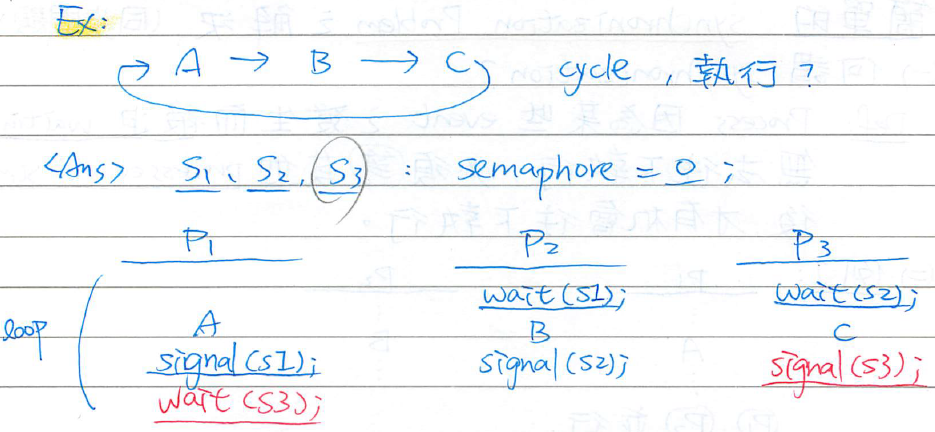
\includegraphics[scale=0.75]{img/ex_semaphore.png}
            \caption{Example of semaphore.}
            \label{img:ex_semaphore}
        \end{figure}
    \end{itemize}
\end{theorem}

\begin{theorem}{(168)} Producer-consumer problem:\begin{itemize}
        \item 共享變數:\begin{lstlisting}[caption={Shared variables of Producer-consumer problem.}, captionpos=b, mathescape=true]
            semaphore mutex := $1$
            semaphore empty := $n$ // buffer空格數。
            semaphore full := $0$ // buffer中item數。
        \end{lstlisting}
        \item 若將其中一個或兩個程式的兩行\code{wait}對調,可能會deadlock。
        \begin{algorithm}[H]
            \caption{Producer.}
            \begin{algorithmic}[1]
                \Function{Producer}{}
                    \Repeat
                        \State Produce an item.
                        \State \Call{wait}{$empty$}
                        \State \Call{wait}{$mutex$}
                        \State Add the item to buffer.
                        \State \Call{signal}{$mutex$}
                        \State \Call{signal}{$full$}
                    \Until {$False$}
                \EndFunction
            \end{algorithmic}
        \end{algorithm}
        \begin{algorithm}[H]
            \caption{Consumer.}
            \begin{algorithmic}[1]
                \Function{Consumer}{}
                    \Repeat
                        \State \Call{wait}{$full$}
                        \State \Call{wait}{$mutex$}
                        \State Retrieve an item from buffer.
                        \State \Call{signal}{$mutex$}
                        \State \Call{signal}{$empty$}
                        \State Consume the item.
                    \Until {$False$}
                \EndFunction
            \end{algorithmic}
        \end{algorithm}
    \end{itemize}
\end{theorem}

\begin{theorem}{(182)} Reader/Writer problem:\begin{itemize}
        \item Reader和writer以及writer和writer皆要互斥。
        \item First readers/writers problem:\begin{itemize}
            \item 共享變數:\begin{lstlisting}[caption={Shared variables of First Reader/Writer problem.}, captionpos=b, mathescape=true]
                // R/W和W/W互斥控制,同時對writer不利之阻擋。
                semaphore wrt := $1$ 
                int readcnt := $0$
                semaphore mutex := $1$ // readcnt互斥控制。
            \end{lstlisting}
        \end{itemize}
        \begin{algorithm}[H]
            \caption{Writer (First Reader/Writer problem).}
            \begin{algorithmic}[1]
                \Function{Writer}{}
                    \Repeat
                        \State \Call{wait}{$wrt$}
                        \State Writing.
                        \State \Call{signal}{$wrt$}
                    \Until {$False$}
                \EndFunction
            \end{algorithmic}
        \end{algorithm}
        \begin{algorithm}[H]
            \caption{Reader (First Reader/Writer problem).}
            \begin{algorithmic}[1]
                \Function{Reader}{}
                    \Repeat
                        \State \Call{wait}{$mutex$}
                        \State $readcnt$ := $readcnt + 1$
                        \If {$readcnt = 1$} \Comment{表示第一個reader需偵測有無writer在。}
                            \State \Call{wait}{$wrt$} 
                        \EndIf
                        \State \Call{signal}{$mutex$} 
                        \State Reading.
                        \State \Call{wait}{$mutex$}
                        \State $readcnt$ := $readcnt - 1$
                        \If {$readcnt = 0$} \Comment{No reader.}
                            \State \Call{signal}{$wrt$} 
                        \EndIf
                        \State \Call{signal}{$mutex$}
                    \Until {$False$}
                \EndFunction
            \end{algorithmic}
        \end{algorithm}
        \item Second Reader/Writer problem:\begin{itemize}
            \item 共享變數:\begin{lstlisting}[caption={Shared variables of Second Reader/Writer problem.}, captionpos=b, mathescape=true]
                int readcnt := $0$
                semaphore mutex := $1$ // readcnt互斥控制。
                semaphore wrt := $1$ // R/W和W/W互斥控制。
                int wrtcnt := $0$
                semaphore y := $1$ // wrtcnt互斥控制。
                semaphore rsem := $1$ // 對reader不利之阻擋。
                semaphore z := $1$ // reader的入口控制,可有可無。
            \end{lstlisting}
        \end{itemize}
        \begin{algorithm}[H]
            \caption{Writer (Second Reader/Writer problem).}
            \begin{algorithmic}[1]
                \Function{Writer}{}
                    \Repeat
                        \State \Call{wait}{$y$} 
                        \State $wrtcnt$ := $wrtcnt + 1$
                        \If {$wrtcnt = 1$} \Comment{表示第一個writer需阻擋readers。}
                            \State \Call{wait}{rsem}
                        \EndIf
                        \State \Call{signal}{$y$}
                        \State \Call{wait}{$wrt$}
                        \State Writing.
                        \State \Call{wait}{$y$}
                        \State $wrtcnt$ := $wrtcnt - 1$
                        \If {$wrtcnt = 0$}
                            \State \Call{signal}{rsem} \Comment{No writer.}
                        \EndIf
                        \State \Call{signal}{$wrt$}
                        \State \Call{signal}{$y$}
                    \Until {$False$}
                \EndFunction
            \end{algorithmic}
        \end{algorithm}
        \begin{algorithm}[H]
            \caption{Reader (Second Reader/Writer problem).}
            \begin{algorithmic}[1]
                \Function{Reader}{}
                    \Repeat
                        \State \Call{wait}{$z$} 
                        \State \Call{wait}{$rsem$} 
                        \State \Call{wait}{$mutex$}
                        \State $readcnt$ := $readcnt + 1$
                        \If {$readcnt = 1$}
                            \State \Call{wait}{$wrt$}
                        \EndIf
                        \State \Call{signal}{$mutex$}
                        \State \Call{signal}{$rsem$} 
                        \State \Call{signal}{$z$} 
                        \State Reading.
                        \State \Call{wait}{$mutex$}
                        \State $readcnt$ := $readcnt - 1$
                        \If {$readcnt = 0$}
                            \State \Call{signal}{$wrt$}
                        \EndIf
                        \State \Call{signal}{$mutex$}
                    \Until {$False$}
                \EndFunction
            \end{algorithmic}
        \end{algorithm}
    \end{itemize}
\end{theorem}

\begin{theorem}{(184)} The sleeping barber problem:\begin{itemize}
        \item 共享變數:\begin{lstlisting}[caption={Shared variables of The sleeping barber problem.}, captionpos=b, mathescape=true]
            semaphore customer := $0$ // 強迫barber sleep。
            // 強迫customer sleep if barber is busy。
            semaphore barber := $0$ 
            int waiting := $0$ // 正在等待的customers個數。
            semaphore mutex := $1$ // waiting互斥控制。
        \end{lstlisting}
        \item 若將\textsc{Barber}將兩行\code{wait}對調,可能會deadlock。
        \begin{algorithm}[H]
            \caption{Barber.}
            \begin{algorithmic}[1]
                \Function{Barber}{}
                    \Repeat
                        \State \Call{wait}{$customer$} \Comment{Barber go to sleep if no customer.}
                        \State \Call{wait}{$mutex$}
                        \State $waiting$ := $waiting - 1$
                        \State \Call{signal}{$barber$} \Comment{Wake up customer.}
                        \State \Call{signal}{$mutex$}
                        \State Cutting hair.
                    \Until {$False$}
                \EndFunction
            \end{algorithmic}
        \end{algorithm}
        \begin{algorithm}[H]
            \caption{Customer.}
            \begin{algorithmic}[1]
                \Function{Customer}{}
                    \Repeat
                        \State \Call{wait}{$mutex$}
                        \If {$waiting < n$} \Comment{入店。}
                            \State $waiting$ := $waiting + 1$
                            \State \Call{signal}{$mutex$}
                            \State \Call{signal}{$customer$} \Comment{Wake up barber.}
                            \State \Call{wait}{$barber$} \Comment{Customer go to sleep if barber is busy.}
                            \State Getting cut.
                        \Else
                            \State \Call{signal}{$mutex$}
                        \EndIf
                    \Until {$False$}
                \EndFunction
            \end{algorithmic}
        \end{algorithm}
    \end{itemize}
\end{theorem}

\begin{theorem}{(187)} The dining-philosophers problem:\begin{itemize}
        \item 五位哲學家兩兩間放一根筷子吃中餐(筷子),哲學家需取得左右兩根筷子才能吃飯。若吃西餐(刀叉),必須偶數個哲學家,
        \item Algorithm 1(錯誤):\begin{itemize}
            \item 共享變數:\begin{lstlisting}[caption={Shared variables of The dining-philosophers problem.}, captionpos=b, mathescape=true]
                semaphore chopstick[$0 \ \cdots \ 4$] := $1$
            \end{lstlisting}
            \item 會deadlock,若每位哲學家皆取左手邊的筷子,則每個哲學家皆無法拿起右手邊的筷子。
            \begin{algorithm}[H]
                \caption{Algorithm 1 $P_i$ (The dining-philosophers problem).}
                \label{algo:din-philo-algo-1}
                \begin{algorithmic}[1]
                    \Function{$P_i$}{}
                        \Repeat
                            \State Hungry.
                            \State \Call{wait}{$chopstick[i]$}
                            \State \Call{wait}{$chopstick[(i + 1 \Mod{5})]$}
                            \State Eating.
                            \State \Call{signal}{$chopstick[i]$}
                            \State \Call{signal}{$chopstick[(i + 1 \Mod{5})]$}
                            \State Thinking.
                        \Until {$False$}
                    \EndFunction
                \end{algorithmic}
            \end{algorithm}
        \end{itemize}
        \item Algorithm 2(正確):\begin{itemize}
            \item 根據公式 (\ref{eq:deadlock}),人數必須$< 5$才不會deadlock。
            \item 共享變數:\begin{lstlisting}[caption={Shared variables of The dining-philosophers problem.}, captionpos=b, mathescape=true]
                semaphore chopstick[$0 \ \cdots \ 4$] := $1$ 
                // 可拿筷子的哲學家數量互斥控制。
                semaphore no := $4$ 
            \end{lstlisting}
            \begin{algorithm}[H]
                \caption{Algorithm 2 $P_i$ (The dining-philosophers problem).}
                \begin{algorithmic}[1]
                    \Function{$P_i$}{}
                        \Repeat
                            \State \Call{wait}{$no$}
                            \State (Same as Algorithm 1.) 
                            \State \Call{signal}{$no$}
                        \Until {$False$}
                    \EndFunction
                \end{algorithmic}
            \end{algorithm}
        \end{itemize}
        \item Algorithm 3:只有能夠同時拿左右兩根筷子才允許持有筷子,否則不可持有任何筷子,破除hold and wait,不會deadlock。
        \item Algorithm 4:當有偶數個哲學家時,偶數號的哲學家先取左邊,再取右邊,奇數號的則反之,破除circular waiting,不會deadlock。與吃西餐先拿刀再拿叉相似。
    \end{itemize}
\end{theorem}

\begin{theorem}{()} Binary semaphore製作counting semaphore(若為$-n$表示$n$個process卡在\code{wait}):\begin{itemize}
        \item 共享變數:\begin{lstlisting}[caption={Shared variables of The dining-philosophers problem.}, captionpos=b, mathescape=true]
            int c := $n$ // Counting semaphore號誌值。
            semaphore $s_1$ := $1$ // c互斥控制。
            binary_semaphore $s_2$ := $0$ // $c < 0$時卡住process
        \end{lstlisting}
        \begin{algorithm}[H]
            \caption{$wait(c)$ (counting semaphore).}
            \begin{algorithmic}[1]
                \Function{wait}{$c$}
                    \State \Call{wait}{$s_1$}
                    \State $c$ := $c - 1$
                    \If {$c < 0$}
                        \State \Call{signal}{$s_1$}
                        \State \Call{wait}{$s_2$} \Comment{Process卡住。}
                    \Else
                        \State \Call{signal}{$s_1$}
                    \EndIf
                \EndFunction
            \end{algorithmic}
        \end{algorithm}
        \begin{algorithm}[H]
            \caption{$signal(c)$ (counting semaphore).}
            \begin{algorithmic}[1]
                \Function{signal}{$c$}
                    \State \Call{wait}{$s_1$}
                    \State $c$ := $c + 1$
                    \If {$c \le 0$} \Comment{先前有process卡住。}
                        \State \Call{signal}{$s_2$}
                    \EndIf
                    \State \Call{signal}{$s_1$}
                \EndFunction
            \end{algorithmic}
        \end{algorithm}
    \end{itemize}
\end{theorem}

\begin{theorem}{()} Non-busy waiting semaphore:
    \begin{lstlisting}[caption={Non-busy waiting semaphore.}, captionpos=b]
        struct semaphore {
            int value;
            Queue Q; // Waiting queue.
        }
    \end{lstlisting}
    \begin{algorithm}[H]
        \caption{$wait(S)$ (non-busy waiting semaphore).}
        \begin{algorithmic}[1]
            \Function{wait}{$S$}
                \State $S.value$ := $S.value - 1$
                \If {$S.value < 0$}
                    \State Add process $p$ into $S.Q$.
                    \State $block(p)$ \Comment{System call將$p$的state從running改為wait,有context switch cost。}
                \EndIf
            \EndFunction
        \end{algorithmic}
    \end{algorithm}
    \begin{algorithm}[H]
        \caption{$signal(S)$ (non-busy waiting semaphore).}
        \begin{algorithmic}[1]
            \Function{signal}{$S$}
                \State $S.value$ := $S.value + 1$
                \If {$S.value \le 0$}
                    \State Remove process $p$ from $S.Q$.
                    \State $wakeup(p)$ \Comment{System call將$p$的state從wait改為ready,有context switch cost。}
                \EndIf
            \EndFunction
        \end{algorithmic}
    \end{algorithm}
\end{theorem}

\begin{theorem}{()} 製作semaphore:\begin{itemize}
        \item Algorithm 1 (disable interrupt and non-busy waiting):\label{algo:inter-non-busy}
        \begin{algorithm}[H]
            \caption{$wait(S)$ of Algorithm 1 (disable interrupt and non-busy waiting).}
            \begin{algorithmic}[1]
                \Function{wait}{$S$}
                    \State Disable interrupt.
                    \State $S.value$ := $S.value - 1$
                    \If {$S.value < 0$}
                        \State Add process $p$ into $S.Q$.
                        \State Enable interrupt.
                        \State $block(p)$ 
                    \Else 
                        \State Disable interrupt.
                    \EndIf
                \EndFunction
            \end{algorithmic}
        \end{algorithm}
        \begin{algorithm}[H]
            \caption{$signal(S)$ of Algorithm 1 (disable interrupt and non-busy waiting).}
            \begin{algorithmic}[1]
                \Function{signal}{$S$}
                    \State Disable interrupt.
                    \State $S.value$ := $S.value + 1$
                    \If {$S.value \le 0$}
                        \State Remove process $p$ from $S.Q$.
                        \State $wakeup(p)$ \Comment{System call將$p$的state從wait改為ready,有context switch cost。}
                    \EndIf
                    \State Enable interrupt.
                \EndFunction
            \end{algorithmic}
        \end{algorithm}
        \item Algorithm 2 (critacal section design and non-busy waiting):\label{algo:cs-non-busy}將Algorithm 1 (\ref{algo:inter-non-busy})中的\code{Enable interrupt.}和\code{Disable interrupt.}分別改為\code{Entry section.}和\code{Exit section.}並使用\textsc{Test-and-Set} (\ref{algo:test-and-set-algo-2})或\textsc{Compare-and-Swap} (\ref{algo:comp-and-swap})實現。
        \item Algorithm 3 (disable interrupt design and busy waiting):\label{algo:inter-busy}
        \begin{algorithm}[H]
            \caption{$wait(S)$ of Algorithm 3 (disable interrupt design and busy waiting).}
            \begin{algorithmic}[1]
                \Function{wait}{$S$}
                    \State Disable interrupt.
                    \While {$S \le 0$}
                        \State Enable interrupt.
                        \State Nop.
                        \State Disable interrupt.
                    \EndWhile
                    \State $S$ := $S - 1$ 
                    \State Enable interrupt.
                \EndFunction
            \end{algorithmic}
        \end{algorithm}
        \begin{algorithm}[H]
            \caption{$signal(S)$ of Algorithm 3 (disable interrupt design and busy waiting).}
            \begin{algorithmic}[1]
                \Function{signal}{$S$}
                    \State Disable interrupt.
                    \State $S$ := $S + 1$
                    \State Enable interrupt.
                \EndFunction
            \end{algorithmic}
        \end{algorithm}
        \item Algorithm 4 (critical section design and busy waiting):同Algorithm 2 (\ref{algo:cs-non-busy}),將Algorithm 3 (\ref{algo:inter-busy})中的\code{Enable interrupt.}和\code{Disable interrupt.}分別改為\code{Entry section.}和\code{Exit section.}。
    \end{itemize}
\end{theorem}

\subsubsection{Monitor}

\begin{theorem}{(189)} Monitor:\begin{itemize}
        \item High-level abstraction, belongs to programming language.
        \item Definition:\begin{itemize}
            \item Shared variables.
            \item A set of functions.
            \item Initialization code.
        \end{itemize} 
        \item 只有monitor內functions可以直接存取shared memory。
        \item Monitor本身確保mutual exclusion,同一時間最多允許一個process呼叫monitor的任一function。
        \item Programmer不需煩惱shared variables的race condition problem,只需解決synchronization problem。
        \item Condition variables:在monitor內的condition type變數,用以解決synchronization problem。提供member functions:\begin{itemize}
            \item \code{wait}:Block process放到各自的waiting queue。
            \item \code{signal}:若有process在其waiting queue則恢復該process執行,否則無作用。
            \item \code{wait(c)}:Conditional wait,有時候需要priority queue包含entry和waiting queue,priority越高越先移出,其中$c$表示priority number。
        \end{itemize}
        \item Process is NOT active:\begin{itemize}
            \item Process呼叫的function執行完畢。
            \item Process執行\code{wait()}被blocked。
        \end{itemize}
    \end{itemize}
\end{theorem}

\begin{theorem}{(191)} Monitor解The dining philosophers problem:
    \begin{lstlisting}[caption={Data structure (The dining philosophers problem (Monitor)).}, captionpos=b, mathescape=true]
        Monitor Dining-ph {
            enum {
                thinking, hungry, eating
            } state[5];
        } 
        Condition self[5];
    \end{lstlisting}
    \begin{algorithm}[H]
        \caption{$pickup(i)$.}
        \begin{algorithmic}[1]
            \Function{pickup}{$i$}
                \State $state[i]$ := $hungry$
                \State \Call{test}{i}
                \If {$state[i] \neq eating$}
                    \State \Call{$self[i]$.wait}{}
                \EndIf
            \EndFunction
        \end{algorithmic}
    \end{algorithm}
    \begin{algorithm}[H]
        \caption{$test(i)$.}
        \begin{algorithmic}[1]
            \Function{test}{$i$}
                \If {$state[(i + 4) \Mod{5}] \neq eating \land state[i] = hungry \land state[(i + 1) \Mod{5}] \neq eating$}
                    \State $state[i]$ := $eating$
                    \State \Call{$self[i]$.signal}{}
                \EndIf
            \EndFunction
        \end{algorithmic}
    \end{algorithm}
    \begin{algorithm}[H]
        \caption{$putdown(i)$.}
        \begin{algorithmic}[1]
            \Function{putdown}{$i$}
                \State $state[i]$ := $thinking$
                \State \Call{test}{$(i + 4) \Mod{5}$}
                \State \Call{test}{$(i + 1) \Mod{5}$}
            \EndFunction
        \end{algorithmic}
    \end{algorithm}
    \begin{algorithm}[H]
        \caption{$initialization\_code(i)$.}
        \begin{algorithmic}[1]
            \Function{initialization\_code}{} \Comment{For non-Condition type.}
                \For {$i$ := $0$ to $4$}
                    \State $state[i]$ := $thinking$
                \EndFor
            \EndFunction
        \end{algorithmic}
    \end{algorithm}
    \begin{algorithm}[H]
        \caption{$P_i$ (The dining philosophers problem (Monitor)).}
        \begin{algorithmic}[1]
            \Function{$P_i$}{}
                \State Dining\_ph dp \Comment{Shared variable.}
                \Repeat
                    \State Hungry. \Comment{No active.}
                    \State \Call{$dp$.pickup}{$i$} \Comment{Running: active; Blocked: NOT active.}
                    \State Eating. \Comment{No active.}
                    \State \Call{$dp$.putdown}{$i$} \Comment{Active.}
                    \State Thinking. \Comment{No active.}
                \Until {$False$}
            \EndFunction
        \end{algorithmic}
    \end{algorithm}
\end{theorem}

\begin{theorem}{()} Example of monitor:若有三台printers,且process ID越小,priority越高。
    \begin{lstlisting}[caption={Data structure of example of monitor)}, captionpos=b, mathescape=true]
        Monitor PrinterAllocation {
            bool pr[3];
            Condition x;
        } 
    \end{lstlisting}
    \begin{algorithm}[H]
        \caption{$Apply(i)$.}
        \begin{algorithmic}[1]
            \Function{Apply}{$i$}
                \If {$pr[0] \land pr[1] \land pr[2]$}
                    \State \Call{$x$.wait}{$i$}
                \Else
                    \State $n$ := Non-busy printer
                    \State $pr[n]$ := $True$
                    \State \Return $n$
                \EndIf
            \EndFunction
        \end{algorithmic}
    \end{algorithm}
    \begin{algorithm}[H]
        \caption{$Release()$.}
        \begin{algorithmic}[1]
            \Function{Release}{$n$}
                \State $pr[n]$ := $False$
                \State \Call{$x$.signal}{}
            \EndFunction
        \end{algorithmic}
    \end{algorithm}
    \begin{algorithm}[H]
        \caption{$initialization\_code()$.}
        \begin{algorithmic}[1]
            \Function{initialization\_code}{}
                \For {$i$ := $0$ to $2$}
                    \State $pr[i]$ := $False$
                \EndFor
            \EndFunction
        \end{algorithmic}
    \end{algorithm}
    \begin{algorithm}[H]
        \caption{$P_i$ of example of monitor.}
        \begin{algorithmic}[1]
            \Function{$P_i$}{}
                \State $pa$ := \Call{PrinterAllocation}{}  \Comment{Shared variable.}
                \State $n$ := \Call{$pa$.Apply}{$i$}
                \State Using printer $pr[n]$ .
                \State \Call{$pa$.Release}{$n$}
            \EndFunction
        \end{algorithmic}
    \end{algorithm}
\end{theorem}

\begin{theorem}{()} 使用Monitor製作binary semaphore:
    \begin{lstlisting}[caption={Data structure (Making semaphore using monitor).}, captionpos=b, mathescape=true]
        Monitor Semaphore {
            int value;
            Condition x;
        }
    \end{lstlisting}
    \begin{algorithm}[H]
        \caption{$Wait()$.}
        \begin{algorithmic}[1]
            \Function{Wait}{}
                \If {$value \le 0$}
                    \State \Call{$x$.wait}{}
                \EndIf
                \State $value$ := $value - 1$
            \EndFunction
        \end{algorithmic}
    \end{algorithm}
    \begin{algorithm}[H]
        \caption{$Signal()$.}
        \begin{algorithmic}[1]
            \Function{Signal}{}
                \State $value$ := $value + 1$
                \State \Call{$x$.signal}{}
            \EndFunction
        \end{algorithmic}
    \end{algorithm}
    \begin{algorithm}[H]
        \caption{$initialization\_code()$.}
        \begin{algorithmic}[1]
            \Function{initialization\_code}{}
                \State $value$ := $1$
            \EndFunction
        \end{algorithmic}
    \end{algorithm}
\end{theorem}

\begin{theorem}{()} Monitor種類:Process $P$ call \code{signal}將process $Q$恢復執行,則\begin{itemize}
        \item \begin{itemize}
            \item Type 1:$P$ waits $Q$ until $Q$ finished or $Q$ is blocked again,多一個儲存這種$P$的queue。又稱Hoare monitor。
            \item Type 2:$Q$ waits $P$ until $P$ finished or $P$ is blocked. 不保證$Q$可以resume execution,因為$P$繼續執行很有可能改變$Q$可以恢復執行的條件。
            \item Type 3:$P$先離開,放到entry queue的第一位。保證$Q$一定可以恢復執行,但NOT powerful than Hoare monitor,因為只能一進一出。
        \end{itemize}
        \item \begin{itemize}
            \item signal-and-wait:Type 1, Type 3.
            \item signal-and-continue: Type 2.
        \end{itemize}
    \end{itemize}
\end{theorem}

\begin{theorem}{()} 使用semaphore製作monitor:\begin{itemize}
        \item 共享變數:\begin{lstlisting}[caption={Shared variables of making monitor using semaphore.}, captionpos=b, mathescape=true]
            semaphore mutex := $1$
            // Block process P if P call signal. 
            semaphore next := $0$
            // 統計process P 那種特殊waiting processes的個數。 
            int next_cnt := $0$ 
            // Block process Q if Q call wait.
            semaphore x_sem := $0$ 
            // 統計一般waiting processes的個數。
            int x_cnt := $0$ 
        \end{lstlisting}
        \item 在functions body前後加入控制碼,類似Entry section和Exit section。
        \begin{algorithm}[H]
            \caption{$f$ (Example for adding control code before and after function body).}
            \begin{algorithmic}[1]
                \Function{f}{}
                    \State \Call{wait}{$mutex$}
                    \State Function body.
                    \If {$next\_cnt > 0$}
                        \State \Call{signal}{$next$}
                    \Else
                        \State \Call{signal}{$mutex$}
                    \EndIf
                \EndFunction
            \end{algorithmic}
        \end{algorithm}
        \begin{algorithm}[H]
            \caption{$x.wait()$.}
            \begin{algorithmic}[1]
                \Function{$x$.wait}{}
                    \State $x\_cnt$ := $x\_cnt + 1$
                    \If {$next\_cnt > 0$}
                        \State \Call{signal}{$next$}
                    \Else
                        \State \Call{signal}{$mutex$}
                    \EndIf
                    \State \Call{wait}{$x\_sem$} \Comment{$Q$自己卡住。}
                    \State $x\_cnt$ := $x\_cnt - 1$ \Comment{$Q$被救。}
                \EndFunction
            \end{algorithmic}
        \end{algorithm}
        \begin{algorithm}[H]
            \caption{$x.signal()$.}
            \begin{algorithmic}[1]
                \Function{$x$.signal}{}
                    \If {$x\_cnt > 0$}
                        \State $next\_cnt$ := $next\_cnt + 1$
                        \State \Call{signal}{$x\_sem$}
                        \State \Call{wait}{$next$} \Comment{$P$自己卡住。}
                        \State $next\_cnt$ := $next\_cnt - 1$ \Comment{$P$被救。}
                    \EndIf
                \EndFunction
            \end{algorithmic}
        \end{algorithm}
    \end{itemize}
\end{theorem}

\begin{theorem}{()} 因為monitor和semaphore可以互相製作,所以解決synchronization problem能力相同。
\end{theorem}

\begin{theorem}{(195)} Indirect communication通過shared mailbox;溝通雙方可多條communication links且可與其他processes共享,direct則否。
\end{theorem}

\begin{theorem}{(197)} Link capacity:\begin{itemize}
        \item 每一條communication link皆有一個messages queue,而queue size即link capacity。
        \item receiver:收到訊息才能往下執行;Sender:由link capacity決定synchronization mode (zero (rendezvous,即雙方都在等), bounded, unbounded capacity)。
    \end{itemize}
\end{theorem}
